% !TeX root = er.tex

\chapter{Apprentissage automatique}\label{ch.machine}

Considérons un robot qui reconnaît et saisit des objets jaunes (Fig.~\ref{fig.sortballs}). Il peut utiliser une caméra couleur pour identifier les objets jaunes, mais les objets apparaîtront différemment selon l'environnement, par exemple à la lumière du soleil, dans une pièce sombre ou dans une salle d'exposition. En outre, il est difficile de définir précisément ce que signifie "jaune" : quelle est la frontière entre le jaune et le jaune citron ou entre le jaune et l'orange ? Plutôt que d'écrire des instructions détaillées pour le robot, nous préférerions que le robot apprenne la reconnaissance des couleurs au fur et à mesure qu'il exécute sa tâche, afin qu'il puisse s'adapter à l'environnement dans lequel il opère. Plus précisément, nous voulons concevoir un \emph{algorithme de classification}\index{algorithme de classification} qui peut être \emph{entraîné} à effectuer la tâche sans fournir tous les détails à l'avance.

\begin{figure}
\begin{center}
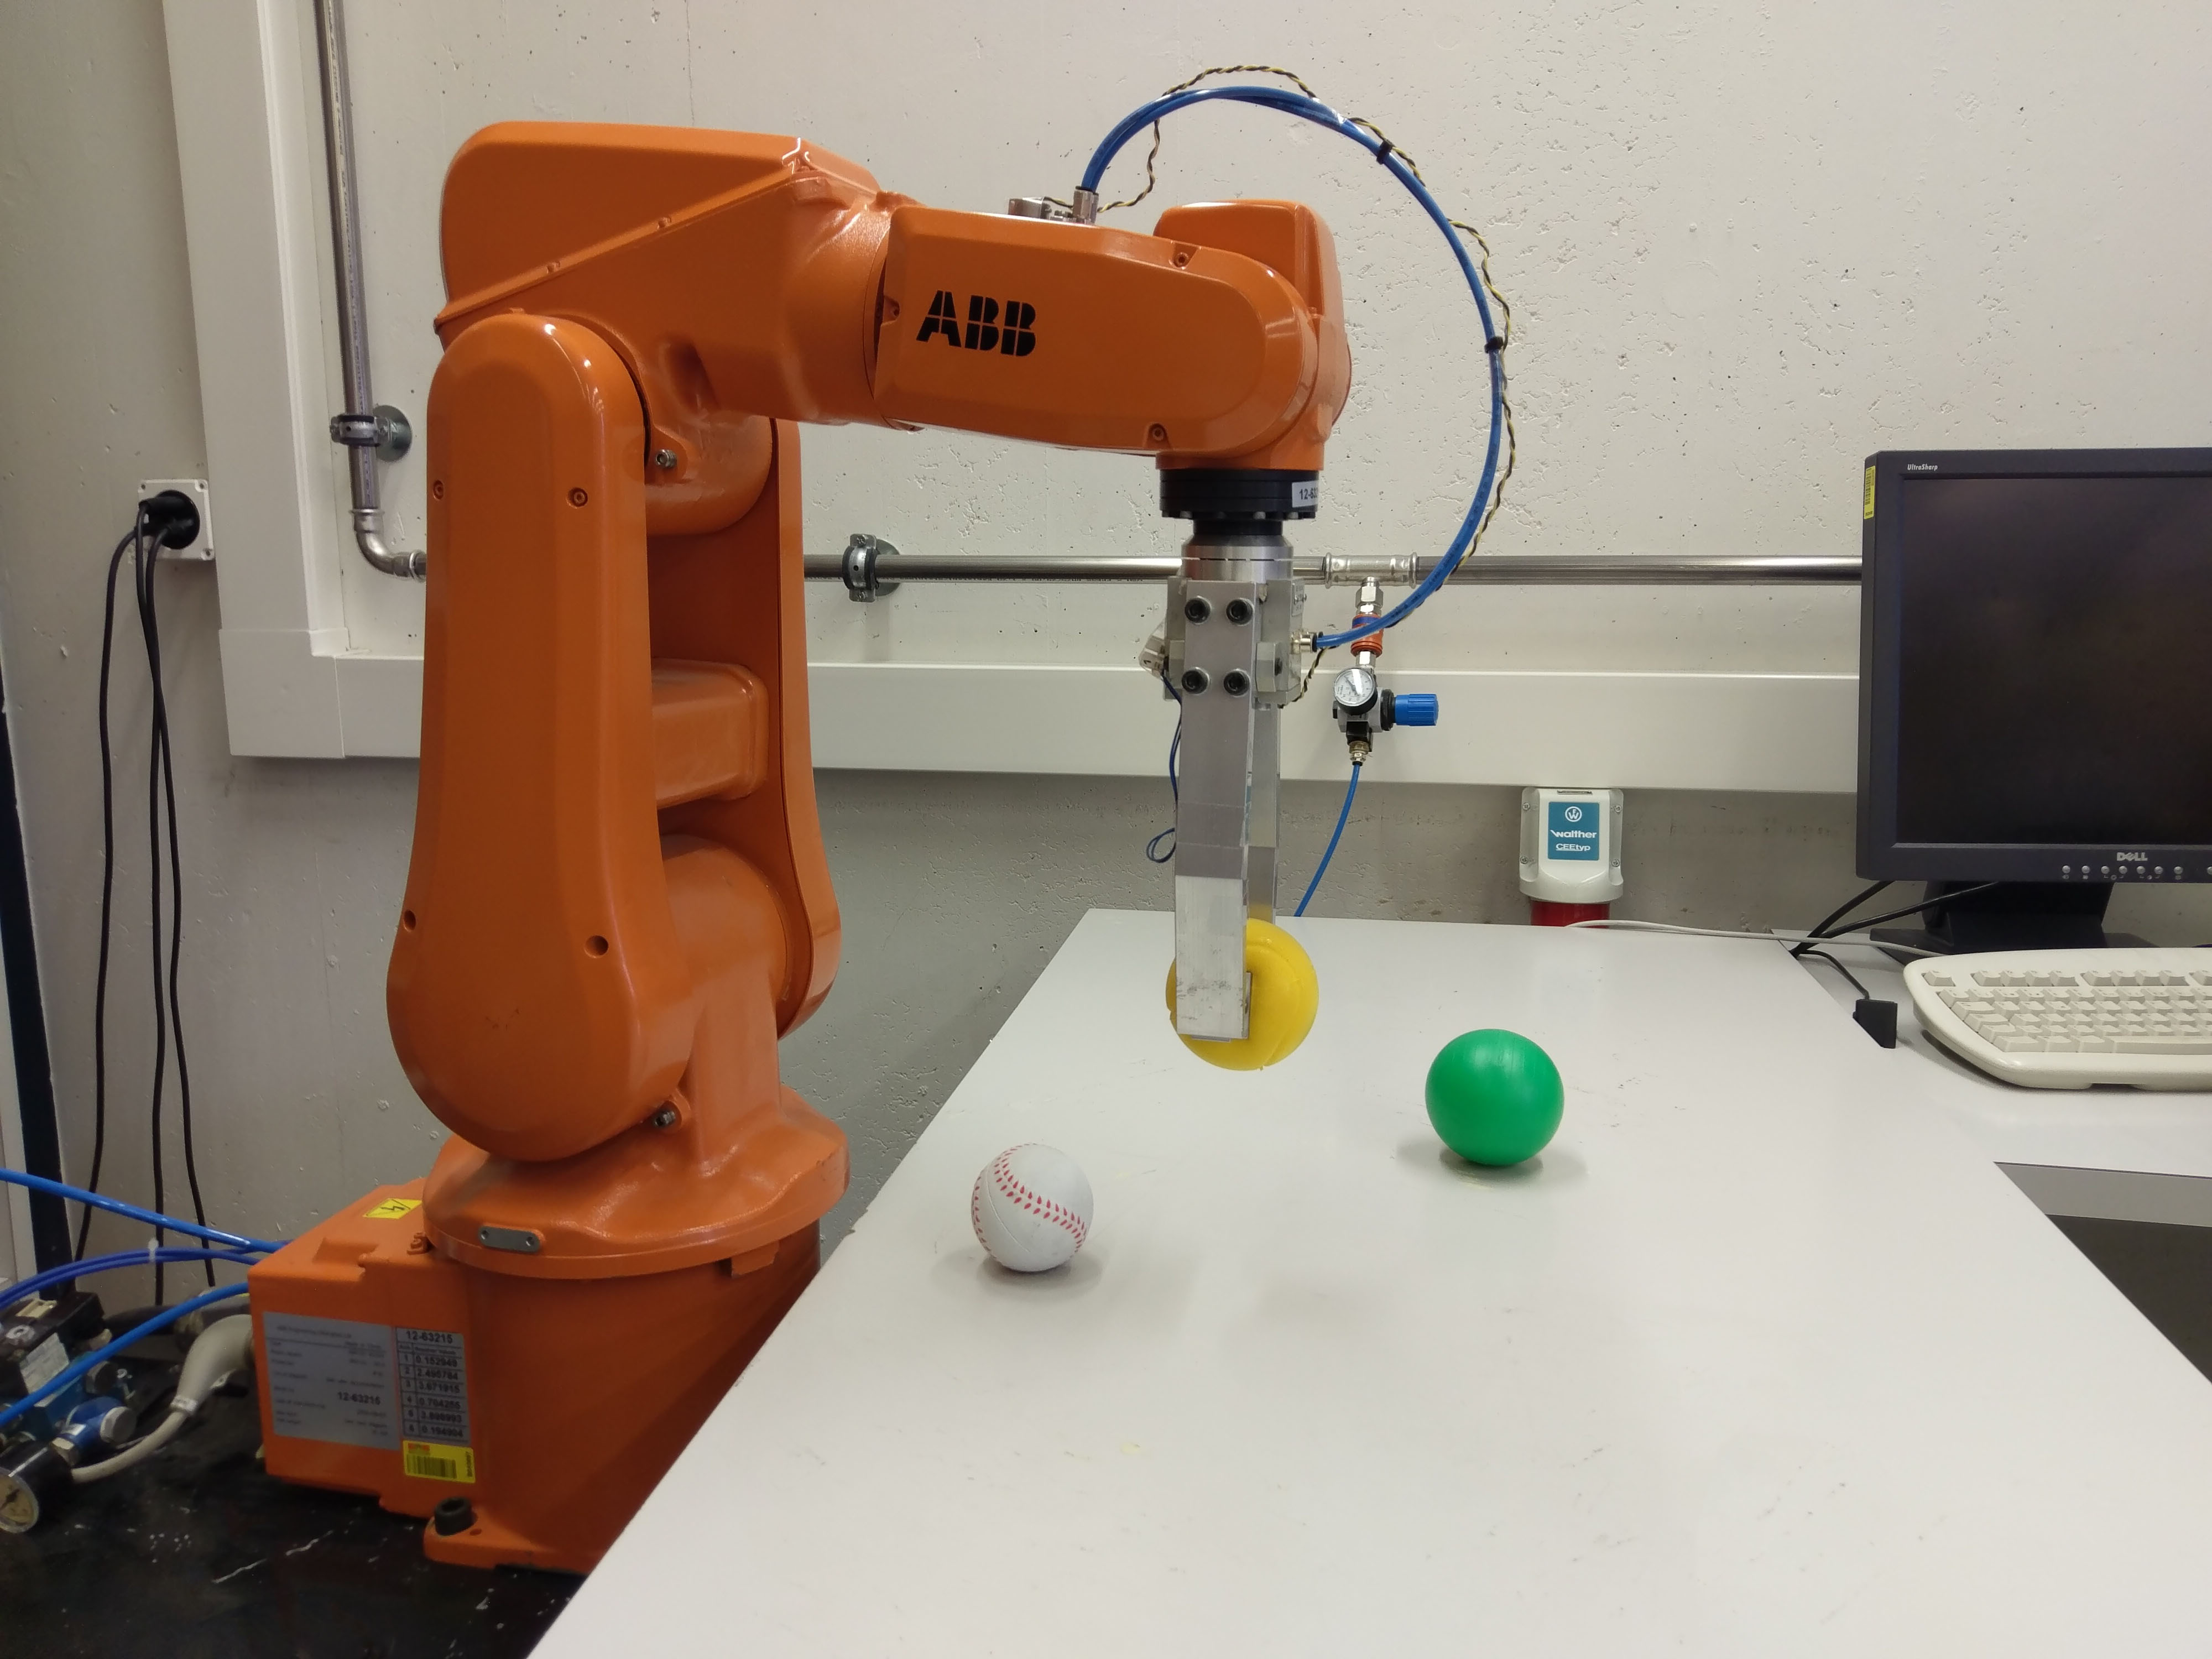
\includegraphics[width=0.8\textwidth]{sorting-robot.jpg}
\end{center}
\caption{Bras robotique triant des balles colorées}\label{fig.sortballs}
\end{figure}

Les algorithmes de classification sont un sujet central de l'apprentissage automatique, un domaine de l'informatique et des statistiques qui développe des méthodes de calculs pour reconnaître des modèles et prédire des résultats sans programmation explicite. Ces algorithmes extraient des \emph{règles} des données brutes acquises par le système au cours d'une période de formation. Les règles sont ensuite utilisées pour classer un nouvel objet et agir de manière appropriées en fonction de la classe de l'objet. Pour la tâche de reconnaissance des couleurs, nous entraînons le robot en lui présentant des objets de différentes couleurs et en lui disant quels objets sont jaunes et lesquels ne le sont pas. L'algorithme d'apprentissage automatique génère une règle de classification des couleurs. Lorsqu'on lui présente de nouveaux objets, il utilise la règle pour décider quels objets sont jaunes et lesquels ne le sont pas.

Le chapitre précédent a présenté les réseaux de neurones artificiels qui réalisent une forme d'apprentissage automatique sur lesquelles reposen le renforcement. Dans ce chapitre, nous abordons les techniques statistiques basées sur l'apprentissage supervisé : pendant la période d'apprentissage, nous donnons au robot des réponses précises, par exemple si un objet est jaune ou non. La section~\ref{s.sorting-onesensor} introduit les techniques statistiques en développant un algorithme permettant de distinguer des objets de deux couleurs. Nous présentons une technique d'apprentissage automatique appelée \emph{analyse discriminante linéaire (LDA)}. Les sections~\ref{s.lda}--\ref{s.gen-lda} présentent la LDA dans le même contexte: faire la distinction entre deux couleurs. L'LDA repose sur l'hypothèse que les données possèdent des propriétés statistiques spécifiques ; si ce n'est pas le cas, les algorithmes de type \emph{perceptrons} peuvent être utilisé pour la classification, comme décrit dans la section~\ref{s.perceptrons}.

Dans ce chapitre suppose que vous connaissez les concepts de \emph{moyenne}, \emph{variance} et \emph{covariance}. Des tutoriels sur ces concepts apparaissent dans les annexes~\ref{a.mean}--\ref{a.covariance}.

\section{Faire la distinction entre deux couleurs}\label{s.sorting-onesensor}

Nous commençons par le problème de la distinction entre des balles jaunes et des balles qui ne sont pas jaunes. Pour simplifier, nous modifions le problème. Il s’agit de distingue les zones gris foncé des zones gris clair imprimées sur du papier collé au sol (Fig.~\ref{fig.closegrays1}). Le robot utilise deux capteurs au sol qui échantillonnent la lumière réfléchie lorsqu'il parcourte les deux zones.

\begin{figure}
\begin{center}
\begin{tikzpicture}[scale=.8]
\pic at (-2.2,1) { robot };
\draw[fill,gray] (-1,.6) rectangle +(6pt,8pt);
\draw[fill,gray] (-1,1.2) rectangle +(6pt,8pt);
\draw[fill,color=black!60]  (0,0) rectangle +(3.5,2);
\draw[fill,color=black!20] (4,0) rectangle +(3.5,2);
\end{tikzpicture}
\caption{Distinguer deux nuances de gris}\label{fig.closegrays1}
\end{center}
\end{figure}

La figure~\ref{fig.closegrays2} montre un graphique des valeurs parrelevées lors de l'échantillonnage des deux capteurs.\footnote{Les données utilisées dans ce chapitre sont des données réelles tirées d'une expérience avec le robot Thymio.} Le robot met environ $70$ secondes pour se déplacer de gauche à droite, en échantillonnant la lumière réfléchie une fois par seconde. Il est facile de constater que les données présentent des variations importantes, qui sont probablement dues au bruit des capteurs ou à la qualité de l’impression des zones grises. La variabilité des résultats renvoyés par les deux capteurs est encore plus problématique. Comment le robot peut-il apprendre à distinguer les nuances de gris compte tenu de la variabilité des échantillons et des capteurs ? Nous voulons créer une règle pour automatiser la distinction entre les deux nuances de gris. 

\begin{figure}
\begin{center}
\includegraphics[width=0.8\textwidth]{gray-fig.pdf}
\end{center}
\caption{Graphique de la lumière réfléchie en fonction du temps pour le capteur gauche (en haut) et le capteur droit (en bas)}\label{fig.closegrays2}
\end{figure}

\subsection{Un discriminant basé sur les moyennes}
\index{apprentissage machine!discriminant basé sur les moyennes}

En examinant les graphiques de la Fig.~\ref{fig.closegrays2}, il est facile distinguer les échantillons qui proviennent de la zone gris dark et de ceux qui proviennent de la zone gris light. Pour le capteur de gauche, les valeurs de la zone gris light appartiennent à l'interval [500 ; 550], tandis que celles provenant de la zone gris dark sont dans [410 ; 460]. Pour le capteur droit, les intervalles sont [460 ; 480] et [380 ; 400]. Pour le capteur gauche, c'est un seuil de 480 qui permettrait la distinction clairement entre le gris light du gris dark, tandis que pour le capteur droit, c'est un seuil de 440 qui permettrait la distinction entre le gris light et le gris dark. Comment choisir automatiquement ces valeurs optimales et comment concilier les seuils des deux capteurs ?

Concentrons-nous d'abord sur le capteur gauche. Nous cherchons un \textit{discriminant}\index{discriminant}, une valeur qui distingue les échantillons des deux couleurs. Considérons les valeurs $\mathit{max}_\sub{dark}$, la valeur maximale renvoyée par l'échantillonnage du gris foncé, et $\mathit{min}_{\sub{light}}$, la valeur minimale renvoyée par l'échantillonnage du gris clair. Sous l'hypothèse raisonnable que
$\mathit{max}_\sub{dark} < \mathit{min}_\sub{light}$, toute valeur $x$ telle que $\mathit{max}_\sub{dark} < x < \mathit{min}_\sub{light}$ permet de distinguer les deux nuances de gris. Le point milieu entre les deux valeurs semble offrir le discriminant le plus robuste.

Sur la Fig.~\ref{fig.closegrays2}, nous voyons que $\mathit{max}_\sub{dark}\approx 460$ est relevé  à environ $10$ s et $\mathit{min}_{\sub{light}}\approx 500$ à environ $60$ s, nous choisissons donc leur moyenne $480$ comme discriminant. Bien que cela soit correct pour cet ensemble de données particulier, il n'est généralement pas judicieux d'utiliser les valeurs maximales et minimales car ce pourraient être des \emph{valeurs aberrantes} : des valeurs extrêmes résultant de circonstances inhabituelles, telles qu'un trou dans le papier qui donnerait à tort une valeur très élevée dans la zone gris foncé.

Une meilleure solution consiste à utiliser \emph{toutes} les données et la fonction la plus simple pour cela est la \emph{moyenne} des valeurs. Soit $\mu_{\sub{foncé}}$ la moyenne des échantillons gris foncé et $\mu_{\sub{clair}}$ la moyenne des échantillons gris clair. Un bon discriminant $\Delta$ est le point milieu des deux moyennes :
\begin{displaymath}
\Delta = \frac{\mu_{\sub{dark}} + \mu_{\sub{light}}}{2}\,.
%\label{eq.discriminant}
\end{displaymath}
Pour les données de la Fig.~\ref{fig.closegrays2}, les moyennes pour le capteur de gauche et le discriminant sont:\footnote{Dans ce chapitre, les valeurs seront arrondies à l'entier le plus proche.}
\[
\mu_{\sub{dark}}^{\sub{left}} = 431,\;\;
\mu_{\sub{light}}^{\sub{left}} = 519,\;\;
\Delta^{\sub{left}} = \frac{431+519}{2} = 475\,.
\]
Un calcul similaire permet d'obtenir le discriminant pour le capteur de droite :
\[
\Delta^{\sub{right}} = 425\,.
\]
Afin d'obtenir une reconnaissance optimale, nous voulons un algorithme capable de décider automatiquement lequel des deux discriminants est le meilleur. Il s'agit d'un premier pas vers la méthode décrite dans la section \ref{s.lda}, où un discriminant est calculé en combinant les données des deux capteurs.

Intuitivement, plus la différence entre les moyennes des données relevées dans les des light et dark est grande :
\[
\left|\,\mu_{\sub{dark}}^{\sub{left}} - \mu_{\sub{light}}^{\sub{left}}\,\right|,\;\;\left|\,\mu_{\sub{dark}}^{\sub{right}} - \mu_{\sub{light}}^{\sub{right}}\,\right|\,,
\]
plus il sera facile de placer un discriminant entre les deux classes. La différence entre les moyennes du capteur de gauche ($88$) est un peu plus grande que la différence entre les moyennes du capteur de droite ($84$). Cela nous amène à choisir le discriminant ($475$) calculé à partir des moyennes du capteur gauche. Cependant, d'après le graphique de la figure \ref{fig.closegraysmus}, il semble que ce ne soit pas le meilleur choix en raison de la grande variabilité des valeurs des échantillons issues du capteur gauche.

\begin{figure}
\begin{center}
\includegraphics[width=0.8\textwidth]{gray-fig-mus.pdf}
\end{center}
\caption{Figure~\ref{fig.closegrays2} avec les moyennes (pointillés tirets courts), les variances (crochets), les discriminants (pointillés tirets longs).}\label{fig.closegraysmus}
\end{figure}

\subsection{Un discriminant basé sur les moyennes et les variances}

Un meilleur discriminant peut être obtenu si l'on considère non seulement la différence des moyennes, mais aussi la dispersion des valeurs de l'échantillon autour de la moyenne. C'est ce qu'on appelle la \emph{variance}. La variance $s^2$ d'une série statistique $\{x_1,x_2,\ldots,x_{n-1},x_n\}$ est:\footnote{Appendice~\ref{a.mean} explique pourquoi $n-1$ est utilisé au lieu de $n$.}
\[
s^2 = \frac{1}{n-1} \sum_{i=1}^n (x_i-\mu)^2\,,
\]
où $\mu$ est la moyenne des valeurs de la série.

La variance calcule la moyenne des carrés des écarts de chaque échantillon avec la moyenne de la série. Les écarts sont élevés au carré parce qu’une  peut être supérieure ou inférieure à la moyenne, mais nous voulons une valeur positive qui mesure la dispersion par rapport la moyenne.

Pour les échantillons des zones claires et sombres des capteurs gauche et droit de la Fig. 14.4, les quatre variances sont représentées sur le graphique par des crochets. L’écart entre les moyennes du capteure du capteur de gauche est légèrement supérieure à l’écart des moyennes du capteur de droitee :
\[
\rule[-2ex]{0pt}{6ex}\left|\,\mu_{\sub{dark}}^{\sub{left}}-\mu_{\sub{light}}^{\sub{left}}\,\right| > \rule[-2ex]{0pt}{6ex}\left|\,\mu_{\sub{dark}}^{\sub{right}}-\mu_{\sub{light}}^{\sub{right}}\,\right|\,,
\]
mais les variances du capteur de droite sont beaucoup plus petites que les variances correspondantes du capteur de gauche :
\[
\rule[-2ex]{0pt}{6ex}\left(s_{\sub{dark}}^{\sub{right}}\right)^2
\ll
\rule[-3ex]{0pt}{6ex}\left(s_{\sub{dark}}^{\sub{left}}\right)^2\,,\;\;\;
\rule[-2ex]{0pt}{6ex}\left(s_{\sub{light}}^{\sub{right}}\right)^2
\ll
\rule[-3ex]{0pt}{6ex}\left(s_{\sub{light}}^{\sub{left}}\right)^2\,.
\]
L'utilisation des variances permet une meilleure classification des deux ensembles, car un capteur avec une variance est plus petite, ce qui facilite la classification.

Un bon discriminant peut être obtenu en combinant les informations des moyennes et des variances. La qualité d'un discriminant $J_k$, pour $k=\mathit{left},\mathit{right}$, est donnée par :
\begin{equation}
J_k = \frac{\left(\mu_{\sub{dark}}^k - \mu_{\sub{light}}^k\right)^2}{\left(s_{\sub{dark}}^k\right)^2 + \left(s_{\sub{light}}^k\right)^2}\,.\label{eq.j}
\end{equation}
Pour maximiser $J$, le numérateur - le carré des écarts entre les moyennes - doit être grand et le dénominateur - la somme des variances des échantillons - doit être petit.

Le tableau~\ref{table.mu-s-j} synthétise les résultats pour l'ensemble de données de la Fig.~\ref{fig.closegraysmus}. Le critère de qualité $J$ pour le capteur de droite est beaucoup plus grand que celui du capteur de gauche. Il s'ensuit que le point moyen entre les moyennes du capteur droit :
\[
\Delta^{\sub{right}}=\frac{383+467}{2}=425
\]
est un meilleur discriminant que le point moyen des moyennes du capteur gauche. En considérant uniquement les écarts dse moyennes $|\mu_{\sub{dark}}-\mu_{\sub{light}}|$, qui est légèrement plus grand pour le capteur gauche que pour le capteur droit, on aurait choisi le point moyen du capteur gauche comme discriminant.

\begin{table}
\caption{La différence entre les moyennes et les critères de qualité $J$}
\label{table.mu-s-j}
\begin{tabular}{p{2.5cm}p{3cm}p{3cm}p{3cm}p{3cm}}
\hline
& \multicolumn{2}{r@{\hspace{1em}}}{left} & \multicolumn{2}{r@{\hspace{1em}}}{right} \\
\hline
& \multicolumn{1}{r}{dark} & \multicolumn{1}{r}{light} & \multicolumn{1}{@{\hspace{3em}}r}{dark} & \multicolumn{1}{r}{light}\\
\hline
$\mu$ & \multicolumn{1}{r}{$431$} & \multicolumn{1}{r}{$519$} & \multicolumn{1}{r}{$383$} & \multicolumn{1}{r}{$467$}\\
$s^2$ & \multicolumn{1}{r}{$121$} & \multicolumn{1}{r}{$225$} & \multicolumn{1}{r}{$16$} & \multicolumn{1}{r}{$49$}\\
$|\mu_{\sub{dark}}-\mu_{\sub{light}}|$ & \multicolumn{2}{r}{$88$} & \multicolumn{2}{r}{$84$}\\
$J$ & \multicolumn{2}{r}{$22$} & \multicolumn{2}{r}{$104$}\\
\hline
\end{tabular}
\end{table}

\subsection{Algorithme d'apprentissage de la distinction des couleurs}

Ces calculs sont effectués par le robot lui-même, de sorte que le choix du meilleur discriminant et du meilleur capteur est automatique. Les détails du calcul sont donnés dans Algorithmes~\ref{alg.learning1}--\ref{alg.recognition1}.\footnote{Les variables en gras représentent des vecteurs ou des matrices.}

Il y a deux classes $C_1$, $C_2$ et deux capteurs. Pendant la phase d'apprentissage, le robot échantillonne les zones des deux niveaux de gris indépendamment et calcule ensuite le critère de qualité $J$. L'échantillonnage et le calcul sont effectués pour chaque capteur, soit l'un après l'autre, soit simultanément. Après la phase d'apprentissage, le robot utilise le point moyen des moyennes ayant la plue grande valeur de $J$ pour la reconnaissance des niveaux de gris.

\begin{figure}
\begin{alg}{Distinguer les classes (phase d'apprentissage)}{learning1}
&\idv{}float $\vec{X_1}, \vec{X_2}$&// Sets of samples\\
&\idv{}float $\mu_1,\mu_2$& // Means of $C_1,C_2$\\
&\idv{}float $s_1,s_2$& // Variances of $C_1,C_2$\\
&\idv{}float $\mu[2]$& // Means of $\mu_1,\mu_2$\\
&\idv{}float $J[2]$& // Criteria of quality\\
&\idv{}integer $k$& // Index of max($J[1],J[2]$)\\
\hline
\stl{}&for sensor i=1, 2&\\
\stl{}&\idc{}Collect a set of samples $\vec{X_1}$ from $C_1$&\\
\stl{}&\idc{}Collect a set  of samples $\vec{X_2}$ from $C_2$&\\
\stl{}&\idc{}Compute means $\mu_1$ of $\vec{X_1}$ and $\mu_2$ of $\vec{X_2}$&\\
\stl{}&\idc{}Compute variances $s_1$ of $\vec{X_1}$ and $s_2$ of $\vec{X_2}$&\\
\stl{}&\idc{}Compute the mean $\mu[i] = \displaystyle\frac{\mu_1 + \mu_2}{2}$&\\
\stl{}&\idc{}Compute the criterion $J[i]$ from Eq.~\ref{eq.j}&\\
\stl{}&$k$ \ass index of max($J[1],J[2]$)&\\
\stl{}&Output $\mu[k],k$&\\
\end{alg}
\end{figure}

\begin{figure}
\begin{alg}{Distinguer les classes (phase de reconnaissance)}{recognition1}
&\idv{}float $\mu$ \ass input $\mu[k]$ from the learning phase&\\
&\idv{}float x&\\
\hline
\stl{}&loop&\\
\stl{}&\idc{}$x$ \ass get new sample&\\
\stl{}&\idc{}if $x < \mu$&\\
\stl{}&\idc{}\idc{}assign $x$ to class $C_1$&\\
\stl{}&\idc{}else&\\
\stl{}&\idc{}\idc{}assign $x$ to class $C_2$&\\
\end{alg}
\end{figure}

\begin{framed}
\act{Caméléon robotique}{caméléon}
\begin{itemize}
\item Construisez un environnement similaire à celui de la Fig.~\ref{fig.closegrays1}. Imprimez deux feuilles de papier avec des niveaux de gris uniformes différents et collez-les au sol.
\item Écrivez un programme qui permet au robot se déplacer à une vitesse constante sur une zone de couleur en échantillonnant la lumière réfléchie périodiquement. Répétez l'opération pour l'autre couleur.
\item Représentez les données, calculez les moyennes et le discriminant.
\item Implémentez un programme de classification des mesures du capteur. Lorsque le robot classe une mesure, il affiche la couleur reconnue à la manière d'un caméléon (ou donne un autre retour d'information si le changement de couleur n'est pas possible avec le robot).
\item Appliquez la même méthode avec un deuxième capteur et comparez la séparabilité des classes en utilisant le critère $J$.
\item Répétez l'exercice avec deux niveaux de gris très proches. Qu'observez-vous ?
\end{itemize}
\end{framed}

\section{Analyse discriminante linéaire}\label{s.lda}

Dans la section précédente, nous avons classé des échantillons de deux niveaux de gris en nous basant sur les mesures d'un capteur sur deux ; le capteur a été choisi automatiquement sur la base d'un critère de qualité. Cette approche simple n'est pas optimale. Au lieu de choisir un discriminant basé sur un seul capteur, nous pouvons obtenir une meilleure reconnaissance en combinant les échantillons des deux capteurs. L'une de ces méthodes, appelée \emph{analyse discriminante linéaire (LDA)}, est basée sur les travaux pionniers réalisés en 1936 par le statisticien Ronald A. Fisher.

\subsection{Motivation}

Pour comprendre les avantages de combiner échantillons provenant de deux capteurs, supposons que nous sayon à classer des objets de deux couleurs : \emph{violet électrique (ev)} et \emph{rouge de cadmium (cr)}. Le violet électrique est composé en grande partie de bleu et d'un peu de rouge, tandis que le rouge cadmium est composé en grande partie de rouge et d'un peu de bleu. Deux capteurs sont utilisés : l'un mesure le niveau de rouge et l'autre le niveau de bleu. Pour un ensemble d'échantillons, nous pouvons calculer leurs moyennes $\mu_j^k$ et leurs variances $(s_j^k)^2$, pour $j=\mathit{ev}, \mathit{cr}$, $k=\mathit{bleu}, \mathit{rouge}$.

Le graphique de gauche de la figure \ref{fig.LDAprincipe} montre des échantillons d'objets violet électrique contenus dans une ellipse en pointillés en haut à gauche et des échantillons d'objets rouge cadmium contenus dans une ellipse en pointillés en bas à droite. Les centres des ellipses sont les moyennes car les échantillons sont distribués symétriquement par rapport aux ellipses. Les coordonnées de $\mu_{ev}$ sont $x$ et $y$ où $x$ est la moyenne des valeurs relevées par le capteur rouge pour les objets violet électrique échantillonnés et $y$ la moyenne pour le capteur bleu avec ces mêmes objets. Les moyennes des capteurs lors de l'échantillonnage des objets rouge cadmium sont affichées de la même manière. Il est facile de voir que les objets violets électriques ont plus de bleu (ils ont une ordonnée plus grande), tandis que les objets rouges cadmium ont plus de rouge (leur abscisse est plus grande).

\begin{figure}
\begin{center}
\includegraphics[width=\textwidth]{LDA-principe-colors2.pdf}
\end{center}
\caption{Un discriminant linéaire optimal pour distinguer deux couleurs}\label{fig.LDAprincipe}
\end{figure}

Le diagramme montre qu'il y a une plus grande différence entre les moyennes pour le capteur bleu qu'entre les moyennes pour le capteur rouge. À première vue, on pourrait penser qu'utiliser uniquement le capteur bleu donnerait un meilleur discriminant. Cependant, ce n'est pas le cas : les droites en pointillées montrent que le discriminant rouge seul permet de distinguer complètement le violet électrique du rouge cadmium, tandis que le discriminant bleu seul classe à tort certains échantillons violets électriques en rouge cadmium (certains échantillons sont en dessous de la droite) et classe à tort certains échantillons rouges cadmium en violet électrique (certains échantillons sont au-dessus de la droite).

La raison de ce résultat non intuitif est que le capteur bleu renvoie des valeurs qui sont très dispersées (ont une grande variance), tandis que le capteur rouge renvoie des valeurs qui sont très regroupées (ont une petite variance), et nous avons vu dans la section \ref{s.sorting-onesensor} que la classification est meilleure si la variance est faible. Le graphique de droite de la Fig.~\ref{fig.LDAprincipe} montre qu'en construisant un discriminant à partir des deux capteurs, il est possible de mieux séparer les objets violet électrique des objets rouge cadmium. Le discriminant est toujours représenté par une droite mais elle n’est plus parallèle à l’un des axes. Cette droite est déterminée en utilisant les variances ainsi que les moyennes. La méthode est appelée analyse discriminante linéaire.

\subsection{Le discriminant linéaire}

Figure~\ref{fig.LDAprincipe} est un graphique $x$-$y$ de données échantillonnées à partir de deux capteurs. Les coordonnées de chaque point placé sont les valeurs renvoyées par le capteur rouge en abscisse et le capteur bleu en ordonnée. La Fig.~\ref{fig.gray-x-y} est un graphique représente de la même manière les données des Figs.~\ref{fig.closegrays2}--\ref{fig.closegraysmus} qui ont été collectées lorsque le robot s'est déplacé sur deux zones grises.  Dans ces graphiques, les valeurs des capteurs sont représentées en fonction du temps, mais le temps ne joue aucun rôle dans la classification, si ce n'est pour relier les échantillons qui ont été mesurés au même moment par les deux capteurs.

\begin{figure}
\begin{center}
\includegraphics[width=\textwidth]{gray-level-base.pdf}
\end{center}
\caption{Graphique des niveaux de gris avec des discriminants pour un capteur unique et un discriminant optimal}
\label{fig.gray-x-y}.
\end{figure}

Dans la figure \ref{fig.gray-x-y}, la classification basée uniquement sur le capteur gauche correspond à la droite verticale en pointillés, tandis que la classification basée uniquement sur le capteur droit correspond à la droite horizontale en pointillés. Les droites de séparation horizontale et verticale ne sont pas optimales. Supposons que l'on utilise la classification basée sur le capteur gauche (la droite verticale) et que l'on considère un échantillon pour lequel le capteur gauche renvoie $470$ et le capteur droit $460$. L'échantillon sera classé en gris foncé même si la classification en gris clair est meilleure. Intuitivement, il est clair que la droite oblique en trait pleine du graphique est un discriminant beaucoup plus précis que l'un ou l'autre des deux discriminants basés sur un seul capteur.

Comment un tel discriminant linéaire peut-il être défini mathématiquement afin d'être déterminé automatiquement ?\footnote{La présentation suivante est abstraite et sera plus facile à comprendre si elle est lue en même temps que l'exemple numérique de la section~\ref{s.num-lda}.} L'équation générale d'une droite non vertical dans le plan est $y=mx+a$, où $m$ est la pente ou le coefficient directeur et $a$ l’ordonnée à l’origine. Une équation cartésienne de la de droite est :
\begin{equation}
w_1x_1 + w_2x_2 = c\,,\label{eq.diseq}
\end{equation}
où $x_1$ est la variable pour les valeurs du capteur gauche (axe horizontal), $x_2$ celle pour les valeurs du capteur droit (axe vertical). $c$ est une constante et $w_1,w_2$ sont les coefficients des variables.

Il est pratique de représenter les coefficients sous la forme d'un vecteur colonne :
\[
\vec{w} = \left[ \begin{array}{c} w_1\\w_2 \end{array} \right]\,.
\]
Dans cette représentation, le vecteur $\vec{w}$ est normal à la droite discriminante et permet donc de définir sa pente, tandis que la constante $c$ permet au discriminant d'être n'importe quelle droite de même pente, c'est-à-dire n'importe laquelle du nombre infini de droites parallèles ayant une pente donnée. Une fois la pente de $\vec{w}$ déterminée, $c$ est obtenu en entrant  les coordonnées ($x_1$,$x_2$) d'un point donné dans l'équation \ref{eq.diseq}.

L'analyse discriminante linéaire définit automatiquement le vecteur $\vec{w}$ et la constante $c$ qui génèrent une droite discriminante optimale entre les ensembles de données des deux classes. La première étape consiste à choisir un point sur la droite discriminante. Par ce point, il existe un nombre infini de droites et nous devons choisir la droite dont la pente donne le discriminant optimal. Enfin, la valeur $c$ peut être calculée à partir de la pente et du point choisi. Les sous-sections suivantes décrivent chacune de ces étapes en détail.

\subsection{Choisir un point pour le discriminant linéaire}

Comment choisir un point ? L'analyse discriminante linéaire repose sur l'hypothèse que les valeurs des deux classes ont la même distribution. De manière informelle, lorsque l'on regarde un graphique $x$-$y$, les deux ensembles de points devraient avoir une taille et une forme similaires. Bien qu'il soit presque certain que les distributions ne seront pas exactement les mêmes (disons une distribution gaussienne) parce qu'elles résultent de mesures effectuées dans le monde réel, étant donné que les deux capteurs sont soumis aux mêmes types de variabilité (bruit du capteur, surface inégale du sol), il est probable qu'elles seront similaires.

Si les deux distributions sont similaires, les moyennes des échantillons de chaque capteur seront plus ou moins au même endroit par rapport aux distributions. La moyenne des moyennes de chaque capteur sera équidistante des points correspondants dans les ensembles de données. Le discriminant est choisi pour être une droite qui passe par le point $M$ (Fig.~\ref{fig.gray-x-y}) dont les coordonnées sont :
\[
\left(\,
\frac{\mu_{\sub{light}}^{\sub{left }}+\mu_{\sub{dark}}^{\sub{left }}}{2},\:\frac{\mu_{\sub{light}}^{\sub{right}}+\mu_{\sub{dark}}^{\sub{right}}}{2}
\,\right)\,.
\]

\subsection{Choisir une pente pour le discriminant linéaire}

Une fois que nous avons choisi le point $M$ de la droite discriminante, l'étape suivante consiste à choisir la pente de la droite. D'après la Fig.~\ref{fig.gray-x-y}, nous voyons qu'il existe une infinité de droites passant par le point $M$ qui permettraient de distinguer les deux ensembles d'échantillons. Quelle est la meilleure droite pour les propriétés statistiques de nos données ?

Dans la section \ref{s.sorting-onesensor}, nous avons cherché un moyen de décider entre deux discriminants, où chaque discriminant était une droite parallèle à l'axe $y$ passant par le point moyen entre les moyennes des valeurs renvoyées par un capteur (Fig.\ref{fig.closegraysmus}). La décision était basée sur le critère de qualité $J_k$ (Eq.~\ref{eq.j}, que l'on rappelle ici):
\begin{equation}
J_k = \frac{\left(\mu_{\sub{dark}}^k - \mu_{\sub{light}}^k\right)^2}{\left(s_{\sub{dark}}^k\right)^2 + \left(s_{\sub{light}}^k\right)^2}\,,\label{eq.j-repeat}
\end{equation}
où $k=\textit{gauche},\textit{droite}$. Le discriminant ayant la plus grande valeur de $J_k$ a été choisi. Pour maximiser $J_k$, le numérateur - le carré de la distance entre les moyennes - doit être grand et le dénominateur - les variances des échantillons - doit être petit.

Maintenant, à la place de calculer un critère de qualité basé sur les valeurs renvoyées par chaque capteur séparément, nous voulons plutôt calculer un critère à partir de toutes les valeurs renvoyées par les deux capteurs. La figure~\ref{fig.lda-proj} montre un graphique des valeurs de deux capteurs, où les valeurs d'une classe sont représentées par des carrés rouges et celles de l'autre classe par des cercles bleus. Il est clair qu'il y a un chevauchement important le long des axes et qu'il est impossible de trouver des droites parallèles aux axes qui permettent de distinguer les groupes. Cependant, si nous projetons les groupes de mesures sur une droite de vecteur directeur:
\[
\vec{w} = \left[\begin{array}{c}w_1\\w_2\end{array}\right]\,,
\]
les deux groupes peuvent être distingués par la droite de séparation définie par l'Eq.~\ref{eq.diseq} :
\[
w_1x_1 + w_2x_2 = c\,,
\]
où $c$ est déterminé par un point de la droite de projection situé entre les points rouge et bleu. Par analogie avec l'équation \ref{eq.j-repeat}, nous devons définir un critère de qualité $J(\vec{w})$, de sorte que de plus $J(\vec{w})$ sera grand meilleur sera le choix de la dropte discriminante. Ensuite, nous devons trouver la valeur de $\vec{w}$ qui maximise $J(\vec{w})$ en différenciant cette fonction en cherchant $\vec{w}$ qui annule la dérivée.

\begin{figure}
\begin{center}
\includegraphics[width=0.9\textwidth]{LDA-principe-proj3.pdf}
\end{center}
\caption{Projection des échantillons de deux classes sur une droite de vecteur directeur $\vec{w}$}\label{fig.lda-proj}
\end{figure}

La définition de $J(\vec{w})$ est basée sur les moyennes et les variances des deux classes mais est trop complexe pour ce livre. Nous donnons sans preuve que la valeur de $\vec{w}$ qui maximise $J(\vec{w})$ est :
\begin{equation}
\vec{w} = \vec{S}^{-1}\,(\vec{\mu_{\sub{light}}}-\vec{\mu_{\sub{dark}}})\,,\label{eq.wLDA}
\end{equation}
où :
\[
\renewcommand{\arraystretch}{1.8}
\vec{\mu_{\sub{light}}}=\left[
\begin{array}{c}\mu_{\sub{light}}^{\sub{left}}\\
\mu_{\sub{light}}^{\sub{right}}\end{array}
\right]\,,\;\;\;
\vec{\mu_{\sub{dark}}}=\left[
\begin{array}{c}\mu_{\sub{dark}}^{\sub{left}}\\
\mu_{\sub{dark}}^{\sub{right}}\end{array}\right]
\]
sont les vecteurs moyens des deux classes et $\vec{S}^{-1}$ est l'inverse de la moyenne des matrices de covariance des deux classes:\footnote{Voir Annexe~\ref{a.covariance} pour la définition de la covariance et Sect.~\ref{s.num-lda} pour un exemple numérique qui clarifiera les calculs.}
\[
\renewcommand{\arraystretch}{2.5}
\vec{S} = \frac{1}{2}
\left[\begin{array}{l@{\hspace{.4em}}l}
s^2\left(\vec{x^{\sub{left}}_\sub{light}}\right) &
\textit{cov}\left(\vec{x^{\sub{left}}_\sub{light}},\vec{x^{\sub{right}}_\sub{light}}\right)\\
\textit{cov}\left(\vec{x^{\sub{right}}_\sub{light}},\vec{x^{\sub{left}}_\sub{light}}\right)&
s^2\left(\vec{x^{\sub{right}}_\sub{light}}\right)
\end{array}\right]
+
\]
\[
\renewcommand{\arraystretch}{2.5}
\qquad\frac{1}{2}\left[\begin{array}{l@{\hspace{.4em}}l}
s^2\left(\vec{x^{\sub{left}}_\sub{dark}}\right)&
\textit{cov}\left(\vec{x^{\sub{left}}_\sub{dark}},\vec{x^{\sub{right}}_\sub{dark}}\right)\\
\textit{cov}\left(\vec{x^{\sub{right}}_\sub{dark}},\vec{x^{\sub{left}}_\sub{dark}}\right)&
s^2\left(\vec{x^{\sub{right}}_\sub{dark}}\right)
\end{array}\right].
\]
Par rapport au cas d'un capteur unique $J_k$, les moyennes sont des vecteurs à deux dimensions car nous avons une moyenne pour chacun des capteurs. La somme des variances devient la matrice de covariance, qui prend en compte à la fois les variances de chacun des deux capteurs et les covariances qui expriment la manière dont les deux capteurs sont liés.

Lorsque les valeurs de $M$ et $\vec{w}$ ont été calculées, il ne reste plus qu'à calculer la constante $c$ pour définir complètement la droite discriminante. La phase d'apprentissage de l'algorithme LDA est ainsi terminée. Dans la phase de reconnaissance, le robot utilise la droite définie par $\vec{w}$ et $c$ pour classer les nouveaux échantillons.

Le calcul est formalisé dans les Algorithmes~\ref{alg.learning2}--\ref{alg.recognition2}, où nous voulons distinguer deux classes $C_1, C_2$ en utilisant deux capteurs. Comparons cet algorithme avec l'Algorithme~\ref{alg.learning1} : les deux ensembles d'échantillons $\vec{X_1},\vec{X_2}$ et les moyennes $\vec{\mu_1},\vec{\mu_2}$ et les variances $\vec{s_1},\vec{s_2}$ sont des vecteurs à deux coordonnées, une pour chacun des capteurs.
\begin{figure}
\begin{alg}{Analyse discriminante linéaire (phase d'apprentissage)}{learning2}
&\idv{}float array[n$_1$,2] $\vec{X_1}$&// Samples of first area\\
&\idv{}float array[n$_2$,2] $\vec{X_2}$&// Samples of second area\\
&\idv{}float array[2] $\vec{\mu_1},\vec{\mu_2}$& // Means of $C_1,C_2$\\
&\idv{}float array[2] $\vec{\mu}$& // Mean of the means\\
&\idv{}float array[2] $\vec{s_1},\vec{s_2}$& // Variances of $C_1,C_2$\\
&\idv{}float $cov_1,cov_2$& // Covariances of $C_1,C_2$\\
&\idv{}float array[2] $\vec{S_\sub{inv}}$&// Inverse of average\\
&\idv{}float $c$& // Constant of the line\\
\hline
\stl{}&Collect a set of $n_1$ samples $\vec{X_1}$ from $C_1$&\\
\stl{}&Collect a set  of $n_2$ samples $\vec{X_2}$ from $C_2$&\\
\stl{}&Compute means $\vec{\mu_1}$ of $\vec{X_1}$ and $\vec{\mu_2}$ of $\vec{X_2}$&\\
\stl{}&$\vec{\mu}$ \ass{} $(\vec{\mu_1}+\vec{\mu_2})/2$&\\
\stl{}&Compute variances $\vec{s_1}$ of $\vec{X_1}$ and $\vec{s_2}$ of $\vec{X_2}$&\\
\stl{}&Compute covariances $cov_1,cov_2$ of &\\
&\idc{}\idc{}$\vec{X_1}$ and $\vec{X_2}$&\\
\stl{}&Compute $\vec{S_\sub{inv}}$ of covariance matrix&\\
\stl{}&Compute $\vec{w}$ from Eq.~\ref{eq.wLDA}&\\
\stl{}&Compute point $M$ from $\vec{\mu}$&\\
\stl{}&Compute $c$ from $M$ and $\vec{w}$&\\
\stl{}&Ouptut $\vec{w}$ and $c$&\\
\end{alg}
\end{figure}

\begin{figure}
\begin{alg}{Analyse discriminante linéaire (phase de reconnaissance)}{recognition2}
&\idv{}float $\vec{w}$ \ass input from the learning phase&\\
&\idv{}float $c$ \ass input from the learning phase&\\
&\idv{}float $\vec{x}$&\\
\hline
\stl{}&loop&\\
\stl{}&\idc{}$\vec{x}$ \ass new sample&\\
\stl{}&\idc{}if $\vec{x}\cdot \vec{w} < c$&\\
\stl{}&\idc{}\idc{}assign $\vec{x}$ to class $C_1$&\\
\stl{}&\idc{}else&\\
\stl{}&\idc{}\idc{}assign $\vec{x}$ to class $C_2$&\\
\end{alg}
\end{figure}

\subsection{Calcul d'un discriminant linéaire : exemple numérique}
\label{s.num-lda}

La figure~\ref{fig.gray-close} est un tracé des échantillons provenant de deux capteurs au sol, mesurés lorsqu'un robot se déplace sur deux zones grises très similaires, l'une étant noire à $83,6\%$ et l'autre noire à $85\%$. La nuance est si faiblLes que l'œil humain ne peut distinguer les deux. Le discriminant linéaire calculé en utilisant l'algorithme~\ref{alg.learning2} peut-il faire mieux ?

\begin{figure}
\begin{center}
\includegraphics[width=\textwidth]{close-gray.pdf}
\caption{Zones grises similaires (points noirs pour la zone la plus sombre, droix rouges pour la zone la plus claire)}
\label{fig.gray-close}
\end{center}
\end{figure}

La classe $C_1$ est la zone gris clair et la classe $C_2$ est la zone gris foncé. Les éléments des ensembles de vecteurs $\vec{X_1}[n_1],\vec{X_2}[n_2]$ sont des vecteurs de la forme :
\[
\vec{x}=\left[ \begin{array}{c} x^{\sub{left}} \\ x^{\sub{right}} \end{array} \right]
\]
sont les mesures des capteurs gauche et droit pour les échantillons de taille $n_1=192$ et $n_2=205$.

Nous commençons par calculer les moyennes des données de la Fig.~\ref{fig.gray-close} :
\begin{displaymath}
\begin{array}{ccccc}
\vec{\mu_1} &=& {\displaystyle\frac{1}{192}} \left( \left[ \begin{array}{c} 389\\324 \end{array}\right] + \left[ \begin{array}{c} 390\\323 \end{array}\right] + ... + \left[ \begin{array}{c} 389\\373 \end{array}\right] \right)&\approx&\left[ \begin{array}{c} 400\\339 \end{array}\right]\\
\\
\vec{\mu_2} &=& {\displaystyle\frac{1}{205}} \left( \left[ \begin{array}{c} 358\\297 \end{array}\right] + \left[ \begin{array}{c} 358\\296 \end{array}\right] + ... + \left[ \begin{array}{c} 352\\327 \end{array}\right] \right)&\approx&\left[ \begin{array}{c} 357\\312 \end{array}\right]\,.
\end{array}
\end{displaymath}
Davantage de données ont été prélevés dans la deuxième zone ($205$) que dans la première ($192$), mais cela n'a pas d'importance pour le calcul des moyennes. Comme attendu, les moyennes $\vec{\mu_1}$ des échantillons de la zone gris clair sont légèrement plus élevées (plus de lumière réfléchie) que les moyennes $\vec{\mu_2}$ des échantillons des zones gris foncé. Cependant, les measures du capteur gauche sont systématiquement plus élevées que celles du capteur droit. La figure~\ref{fig.gray-close-mu-lin} montre les données de la figure~\ref{fig.gray-close} avec des lignes pointillées fines indiquant les moyennes. Il y a deux lignes pour chaque zone : la ligne horizontale pour le capteur de droite et la ligne verticale pour le capteur de gauche.

\begin{figure}
\begin{center}
\includegraphics[width=\textwidth]{close-gray-mu-lin.pdf}
\caption{Moyennes pour chaque classe (pointillées fines), droite discriminante LDA (trait plein), droite discriminante qui distingue complètement les classes (pointillése épais).}
\label{fig.gray-close-mu-lin}
\end{center}
\end{figure}

La matrice de covariance est composée des variances de chacun des capteurs et de leur covariance. Pour $i=1,2$ :
\[
\vec{S}_i = \left[
\renewcommand{\arraystretch}{2}
\begin{array}{l@{\hspace{1em}}l}
s^2\left(X_i^{\sub{left}}\right) &
\textit{cov}\left(X_i^{\sub{left}}, X_i^{\sub{right}}\right)\\
\textit{cov}\left(X_i^{\sub{right}},X_i^{\sub{left}}\right)&
s^2\left(X_i^{\sub{right}}\right)
\end{array}
\right]\,.
\]
Pour les données de la Fig.~\ref{fig.gray-close}, les variances des échantillons de la zone gris clair sont :
\begin{eqnarray*}
s^2(X_1^{\sub{left}}) &=& \frac{1}{191} \left((389 - 400)^2 + (390 - 400)^2 + \cdots + (389 - 400)^2 \right) \approx 187 \\
s^2(X_1^{\sub{right}}) &=& \frac{1}{191} \left((324 - 339)^2 + (323 - 339)^2 + ... + (373 - 339)^2 \right) \approx 286\,.
\end{eqnarray*}

L'équation ~\ref{eq.cov} de l'annexe~\ref{a.covariance} est utilisée pour calculer la covariance. La covariance étant symétrique, elle n'est calculée qu'une seule fois.
\begin{eqnarray*}
\textit{cov}(X_1^{\sub{left}}, X_1^{\sub{right}}) &=& \frac{1}{191}(389 - 400)(324 - 339) + ... +\\
&&\qquad (389 - 400)(373 - 339) )\\
&\approx& -118\,.
\end{eqnarray*}
A l'aide des résultats obtenus et en effectuant un calcul similaire pour $X_2$, on obtient les matrices de covariance :
\[
\vec{S}_1 = \left[ \begin{array}{c} 187\\-118\end{array} \begin{array}{c} -118\\286 \end{array}\right]
\hspace{10mm}
\vec{S}_2 = \left[ \begin{array}{c} 161\\44\end{array} \begin{array}{c} 44\\147 \end{array}\right]\,.
\]

L'étape suivante consiste à calculer la moyenne des matrices de covariance :
\[
\mu_{\vec{S}} = 
\frac{1}{2}\left(\left[ \begin{array}{c} 187\\-118\end{array} \begin{array}{c} -118\\286 \end{array}\right]+
\left[ \begin{array}{c} 161\\44\end{array} \begin{array}{c} 44\\147 \end{array}\right]\right) = 
\left[ \begin{array}{c} 174\\-37\end{array} \begin{array}{c} -38\\216 \end{array}\right]\,,
\]
et à trouver son inverse:\footnote{Voir Annexe~\ref{a.matrices}.}
\[
\vec{S}^{-1} = \left[ \begin{array}{c} 0.006\\0.001\end{array} \begin{array}{c} 0.001\\0.005 \end{array}\right]\,.
\]
Nous pouvons maintenant utiliser l'Eq.~\ref{eq.wLDA} pour calculer $\vec{w}$ :
\[
\vec{w} = \left[ \begin{array}{c} 0.006\\0.001\end{array} \begin{array}{c} 0.001\\0.005 \end{array}\right] \cdot \left( \left[ \begin{array}{c} 400\\339 \end{array}\right] - \left[ \begin{array}{c} 357\\313 \end{array} \right] \right) = \left[ \begin{array}{c} 0.28\\0.17 \end{array} \right]\,.
\]
Le vecteur $\vec{w}$ donne la direction de la droite de projection qui est perpendiculaire à la droite discriminante. Nous utilisons maintenant l'Eq.~\ref{eq.diseq}, appelée ici :
\[
w_1x_1 + w_2x_2 = c
\]
pour calculer la constante $c$, en supposant que nous connaissions les coordonnées $(x_1,x_2)$ d'un point. Mais nous avons spécifié que le point moyen entre les moyennes doit être sur la droite discriminante. Ses coordonnées sont :
\[
\vec{\mu} = \frac{1}{2}(\vec{\mu_1} + \vec{\mu_2}) = \frac{1}{2}\left( \left[ \begin{array}{c} 400\\339 \end{array}\right] + \left[ \begin{array}{c} 357\\313 \end{array}\right] \right) \approx \left[ \begin{array}{c} 379\\326 \end{array}\right]\,.
\]
Donc :
\[
c = 0.28 \cdot 379 + 0.17\cdot 326 \approx 162\,,
\]
et l'équation de la droite discriminante est :
\[
0.28 x_1 + 0.17 x_2 = 162\,.
\]
La droite discriminante est représentée en trait plein dans la Fig.~\ref{fig.gray-close-mu-lin}. Etant donné un nouvel échantillon $(a,b)$, comparez la valeur de $0.28a + 0.17b$ à $162$ : si elle est plus grande, l'échantillon est classé comme appartenant à la classe $C_1$ et si elle est plus petite, l'échantillon est classé comme appartenant à la classe $C_2$. 

\subsection{Comparaison de la qualité des discriminants}

Si nous comparons le discriminant linéaire trouvé ci-dessus avec les deux discriminants simples basés sur les moyennes d'un seul capteur, nous constatons une nette amélioration. En raison du chevauchement des classes dans une seule direction, le discriminant simple pour le capteur de droite ne classe correctement que 84,1\% des échantillons, tandis que le discriminant simple pour le capteur de gauche est un peu meilleur, puisqu'il classe correctement 93,7\% des échantillons. Le discriminant linéaire trouvé à l'aide de LDA est meilleur, classant correctement 97,5\% des échantillons.

Il peut être surprenant de constater qu'il existe des droites discriminantes capables de classer correctement la totalité des échantillons ! L'un de ces discriminants est représenté par la droite en pointillése épais de la figure \ref{fig.gray-close-mu-lin}. Pourquoi n'avons-nous pas trouvé ce discriminant avec la LDA ? La LDA suppose que les deux classes ont une distribution similaire (répartition des valeurs) autour de la moyenne et que le discriminant de la LDA est optimal dans cette hypothèse. Pour nos données, certains points de la deuxième classe sont éloignés de la moyenne et les distributions des deux classes sont donc légèrement différentes. Il est difficile de dire si ces échantillons sont des valeurs aberrantes, peut-être causées par un problème lors de l'impression des zones grises sur le papier. Dans ce cas, il est certainement possible qu'un nouvel échantillonnage des deux zones aboutisse à des distributions similaires, ce qui conduirait à une classification correcte par le discriminant de la LDA.

\subsection{Activités pour la LDA}

Les activités relatives à l'analyse linéaire des données sont rassemblées dans cette section.

\begin{framed}
\act{Caméléon robotique avec LDA}{LDAchameleon}
\begin{itemize}
\item Construisez un environnement comme le montre la Fig.~\ref{fig.closegrays1} mais avec deux niveaux de gris très proches l'un de l'autre.
\item Écrivez un programme qui fait que le robot se déplace à une vitesse constante sur la zone d'une couleur et échantillonne la lumière réfléchie périodiquement. Répétez l'opération pour l'autre couleur.
\item Représentez graphiquement les données.
\item Calculer les moyennes, les matrices de covariance et le discriminant. 
\item Implémenter un programme qui classifie les mesures du capteur. Lorsque le robot classe une mesure, il affiche la couleur reconnue (ou un autre retour d'informations si le changement de couleur n'est pas possible).
\end{itemize}
\end{framed}

\begin{framed}
\act{Evitement d'obstacles avec deux capteurs}{LDAobstacle}
\begin{itemize}
\item Figure~\ref{fig.train-data-avoid} montre un robot s'approchant d'un mur. La partie supérieure la figure montre différentes situations dans lesquelles le robot détecte le mur avec ses capteurs de droite ; il doit donc tourner à gauche pour contourner le mur. De même, dans la partie inférieure de la figure, le robot doit tourner à droite.
\item Ecrivez un programme qui enregistre les valeurs des capteurs de droite et de gauche lorsqu'un bouton est pressé. Le programme stocke également l'identité du bouton qui a été pressé ; cela représente la classe que nous recherchons pour l'évitement des obstacles.
\item Entraînez le robot : Placez le robot près d'un mur et exécutez le programme. Appuyez sur le bouton gauche si le robot doit tourner à gauche ou sur le bouton droit si le robot doit tourner à droite. Répétez l'opération plusieurs fois.
\item Représentez les données Tracez provenant des deux capteurs sur un graphique $x$-$y$ et regroupez-les par classe : tourner à droite ou à gauche pour éviter le mur. Vous devriez obtenir un graphique semblable à celui de la Fig.~\ref{fig.machlearnavoid}.
\item Tracez une droite discriminante séparant les deux classes.
\item Quel est le niveau de performance de votre droite discriminante ? Quel pourcentage des échantillons peut-elle classer avec succès ?
\item Calculez le discriminant optimal en utilisant LDA. Quel est son degré de réussite ? Les hypothèses de la LDA sont-elles respectées ?
\end{itemize}
\end{framed}

\begin{figure}
\begin{center}
\begin{tikzpicture}[align=left]
\foreach \angle/\x in { 100/0cm, 120/2cm, 140/4cm, 110/6cm, 100/8cm } {
  \draw[fill] (\x,0) rectangle +(16mm,1mm);
  \pic[rotate=\angle,scale=0.4] at (\x+8mm, -8mm) { robot };
}
\node at (-1,-.5) {\textsf{tourner}\\\textsf{à gauche}};
\foreach \angle/\x in { 70/0cm, 85/2cm, 65/4cm, 85/6cm, 75/8cm } {
  \draw[fill] (\x,-2.5) rectangle +(16mm,1mm);
  \pic[rotate=\angle,scale=0.4] at (\x+8mm, -33mm) { robot };
}
\node at (-1,-3) {\textsf{tourner}\\\textsf{à droite}};
\end{tikzpicture}
\end{center}
\caption{Entraînement à l'évitement d'obstacles}\label{fig.train-data-avoid}
\end{figure}

\begin{figure}
\begin{center}
\includegraphics[width=0.9\textwidth]{avoid-graph-classes.pdf}
\end{center}
\caption{Données sur l'évitement d'obstacles pour la classe "aller à gauche" (croix rouges) et la classe "aller à droite" (triangles noirs).}\label{fig.machlearnavoid}
\end{figure}

\begin{framed}
\act{Suivre un objet}{follow}
\begin{itemize}
\item Ecrivez un programme qui permet au robot de suivre un objet. Le robot avance s'il détecte l'objet devant lui ; il recule s'il est trop près de l'objet. Le robot tourne à droite si l'objet est à sa droite et tourne à gauche si l'objet est à sa gauche.
\item Utilisez deux capteurs pour pouvoir visualiser les données sur un graphique en dimension 2.
\item Relevez et représentez les données comme dans Activity~\ref{act.LDAobstacle}. Le graphique doit être similaire à celui de la Fig.~\ref{fig.machlearnfollow}.
\item Expliquez la classification des échantillons de la Fig.~\ref{fig.machlearnfollow}. Quel est le problème posé par la classification d'un échantillon comme allant vers l'avant ou vers l'arrière ? Pourquoi les échantillons qui vont vers l'avant et vers l'arrière ont-ils des valeurs différentes pour les capteurs de gauche et de droite ?
\item Proposez un algorithme pour classer les quatre situations. Pourriez-vous utiliser une combinaison de séparateurs linéaires ?
\end{itemize}
\end{framed}

\begin{figure}
\begin{center}
\includegraphics[width=\textwidth]{graph-follow-classes.pdf}
\end{center}
\caption{Données acquises lors d'une phase d'apprentissage du suivi d'un objet}\label{fig.machlearnfollow}
\end{figure}

\section{Généralisation du discriminant linéaire}\label{s.gen-lda}

Dans cette section, nous présentons quelques manières d'étendre et d'améliorer l'analyse discriminante linéaire.

Tout d'abord, nous pouvons avoir plus de capteurs. Les mathématiques deviennent plus complexes car avec $n$ capteurs, les vecteurs auront $n$ éléments et la matrice de covariance aura $n\ fois n$ éléments, ce qui nécessite plus de puissance de calcul et plus de mémoire. Au lieu d'une droite discriminante, le discriminant sera un hyperplan de dimension $n-1$. La classification avec de multiples capteurs est utilisée avec les signaux d'électroencéphalographie (EEG) du cerveau afin de contrôler un robot par la seule pensée.

Activité \ref{act.follow} a illustré une autre généralisation : la classification en plus de deux classes. Les discriminants sont utilisés pour classer chaque paire de classes. Supposons que vous ayez trois classes $C_1$, $C_2$ et $C_3$, et des discriminants $\Delta_{12}, \Delta_{13}, \Delta_{23}$. Si un nouvel échantillon est classé dans la classe $C_2$ par $\Delta_{12}$, dans la classe $C_1$ par $\Delta_{12}$, et dans la classe $C_2$ par $\Delta_{23}$, la classification finale de cet échantillon sera dans la classe $C_2$ car davantage de discriminants l'y affectent.

Une troisième généralisation consiste à utiliser une courbe d'ordre supérieur a place d'une droite, par exemple une fonction quadratique. Un discriminant d'ordre supérieur peut séparer des classes dont les ensembles de données ne sont pas de simples amas d'échantillons.

\section{Perceptrons}\label{s.perceptrons}
\index{perceptron}

LDA ne peut distinguer les classes que sous l'hypothèse que les échantillons ont des distributions similaires dans les classes. Dans cette section, nous présentons une autre approche de la classification à l'aide de \emph{perceptrons} qui sont liés aux réseaux neuronaux (Chap.~\ref{ch.neural}). Nous y avons montré comment les règles d'apprentissage peuvent générer des comportements spécifiques reliant les capteurs et les moteurs ; nous montrons ici comment elles peuvent être utilisées pour classer des données dans de classes.

\subsection{Détection d'une pente}\label{s.detect-slope}

Prenons l'exemple d'un robot qui explore un terrain difficile. Il est important que le robot identifie les pentes raides pour ne pas tomber, mais il est difficile de spécifier à l'avance toutes les situations dangereuses car elles dépendent de caractéristiques telles que la géométrie du sol et de ses propriétés (humide/sec, sableux/boueux). A la place, nous souhaitons entraîner le robot à adapter son comportement à différents environnements.

Pour simplifier le problème, supposons que le robot puisse se déplacer uniquement vers l'avant et vers l'arrière et qu'il dispose d'accéléromètres sur deux axes \emph{relatifs au corps du robot} : l'un mesure l'accélération vers l'avant et vers l'arrière, et l'autre mesure l'accélération vers le haut et vers le bas. Un robot immobile sur une surface plane mesurera une accélération nulle vers l'avant et vers l'arrière, et une accélération vers le bas de $9,8$ m/s$^{2}$ due à la gravité. L'accélération gravitationnelle est relativement forte par rapport à l'accélération d'un robot qui se déplace lentement, de sorte que les valeurs relatives de l'accéléromètre le long des deux axes donneront une bonne indication de son comportement.

La figure~\ref{fig.slopes} montre un robot avançant sur une pente. Les valeurs renvoyées par les deux accéléromètres sont similaires, $\mathit{acc}_1\approx \mathit{acc}_2$, nous pouvons en déduire que le robot se trouve sur une pente. Si $\mathit{acc}_2\gg\mathit{acc}_1$, nous en déduirons que le robot se trouve sur un terrain plat car l'accéléromètre haut/bas mesure toute la force de gravité alors que l'accéléromètre avant/arrière ne mesure que la très faible accélération du robot en mouvement. La tâche consiste à faire la distinction entre une position sûre du robot et une position dans laquelle la pente commence à devenir trop raide, de sorte que le robot risque de tomber.

\begin{figure}
\begin{center}
% Robot on slope
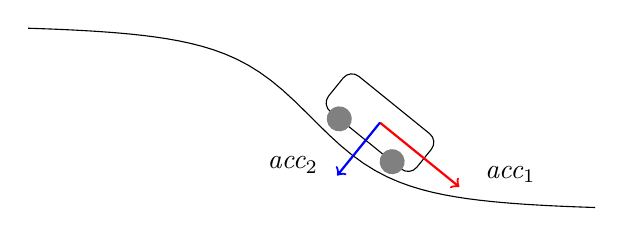
\begin{tikzpicture}[scale=1.2,samples=50,domain=-3:3]
\draw plot (\x,{(-\x/sqrt(\x*\x+1)});
\begin{scope}[xshift=3pt,yshift=4pt,scale=.6,rotate=-39]
\draw[rounded corners] (0,0) -- (0,.8) -- (2, .8) -- (2,0) -- cycle;
\draw[fill,gray] (.4,0) circle[radius=6pt];
\draw[fill,gray] (1.6,0) circle[radius=6pt];
\draw[->,red,thick] (1,.4) -- +(1.8,0);
\draw[->,blue,thick] (1,.4) -- +(0,-1.2);
\end{scope}
\node at (2.1,-.6) {$\textit{acc}_1$};
\node at (-.2,-.5) {$\textit{acc}_2$};
\end{tikzpicture}
\end{center}
\caption{Un robot équipé d'accéléromètres se déplaçant sur un terrain difficile}\label{fig.slopes}
\end{figure}

La figure \ref{fig.slopemes} montre les données acquises au cours d'une session d’entrainement durant laquelle le robot se déplace sur une pente. Lorsque l'opérateur de la session d’entrainement détermine que le robot est stable (classe $C_1$), il lance une mesure indiquée par un croix rouge ; lorsqu'il détermine que le robot est dans une situation dangereuse (classe $C_2$), il lance une mesure indiquée par un triangle noir. Le défi consiste à trouver un moyen de distinguer les échantillons des deux classes.

\begin{figure}
\begin{center}
\includegraphics[width=\textwidth]{slope-allmu.pdf}
\end{center}
\caption{Détection d'une pente dangereuse à l'aide des données des accéléromètres}\label{fig.slopemes}
\end{figure}
Les droites en pointillé de la figure indiquent les moyennes des deux ensembles de données. Il est clair qu'elles ne nous aident pas à classer les données en raison du chevauchement important des deux ensembles. En outre, la méthode LDA n'est pas appropriée car il n'y a pas de similitude dans les distributions : les échantillons lorsque le robot est stable apparaissent dans de nombreuses régions du graphique, tandis que les échantillons provenant de situations dangereuses sont concentrés dans une petite zone autour de leur moyenne.

\subsection{Classification avec perceptrons}
\index{perceptron!classification}

Un \emph{perceptron} est un neurone artificiel doté d'une structure spécifique (Fig.~\ref{fig.perceptron}). Il possède une unité de sommation avec des entrées $\{x_1,\ldots,x_n\}$ et chaque entrée $x_i$ est multipliée par un facteur $w_i$ avant la sommation. Une entrée supplémentaire $x_0$ a une valeur constant égale à $1$ pour créer un biais indépendant des entrées. La sortie du perceptron est obtenue en appliquant une fonction $f$ au résultat de l'addition.

\begin{figure}
\begin{center}
\begin{tikzpicture}%
[node distance=1.5cm and 2cm, nn/.style={circle,draw,minimum size=16pt}]
% Inputs
\node at (0,4) (i1) {};
\node at (0,3) (i2) {};
\node at (0,2) (i3) {};
\node at (0,0) (in) {};
\foreach \y in {.5,.75,1,1.25,1.5} \node at (0,\y) {$.$};
\foreach \i in {i1,i2,i3,in}
  \draw (\i) [yshift=-4pt,xshift=-1pt] arc[start angle=-90, end angle=90, radius=4pt] {};
% Neuron
\pic at (4,2) { nnnode={neuron} };
\% Output
\node (output) [node distance=1.5cm and 1cm,right=of neuron] {};
\draw[->] (neuron) -- (output) node {$y$};
% Arrows to neuron
\draw[->] (i1) node [xshift=-12pt] {$x_0=1$} -- node[fill=white] {$w_0$} (neuron);
\draw[->] (i2) node [xshift=-5pt] {$x_1$} -- node[fill=white] {$w_1$} (neuron);
\draw[->] (i3) node [xshift=-5pt] {$x_2$} -- node[fill=white] {$w_2$} (neuron);
\draw[->] (in) node [xshift=-5pt] {$x_n$} -- node[fill=white] {$w_n$} (neuron);
\end{tikzpicture}
\end{center}
\caption{Un perceptron}\label{fig.perceptron}
\end{figure}

Lorsqu'il est utilisé comme classificateur, les entrées du perceptron sont les valeurs renvoyées par les capteurs pour un échantillon à classer et la sortie sera l'une des deux valeurs indiquant la classe à laquelle l'échantillon est affecté. En général, la fonction de sortie $f$ est simplement le signe de la somme pondérée :
\begin{equation}
y=sign\left(\,\sum_{i=0}^{n} w_i\,x_i\,\right)=\pm 1\,,\label{eq.perceptron-output}
\end{equation}
où une classe correspond à $+1$ et l'autre à $-1$.

Les données sont normalisées de manière à ce que toutes les entrées se situent dans la même plage, généralement $-1\leq x_i\leq +1$. Les données de la figure \ref{fig.slopemes} peuvent être normalisées en divisant chaque valeur par $30$.

Étant donné un ensemble de valeurs d'entrée $\{x_0=1,x_1,\ldots,x_n\}$ d'un échantillon, l'objectif d'une session d'apprentissage est de trouver un ensemble de poids $\{w_0,w_1,\ldots,w_n\}$ de sorte que la sortie soit la valeur $\pm 1$ qui affecte l'échantillon à la bonne classe.

Si l'échantillon est proche de la frontière entre deux classes, la somme pondérée sera proche de zéro. Par conséquent, un perceptron est également un classificateur linéaire : pour distinguer les sorties de $\pm 1$, le discriminant séparant les deux classes est défini par l'ensemble des poids donnant zéro en :
\[
\sum_{i=0}^{n} w_i\,x_i=0\,,
\]
ou
\begin{equation}
w_0 + w_1x_1 + \cdots + w_nx_n = 0\,.\label{eq.perceptron-disc}
\end{equation}
La présentation de la LDA pour un problème bidimensionnel ($n=2$) a conduit à Eq.~\ref{eq.diseq}, qui est la même que Eq.~\ref{eq.perceptron-disc} lorsque $c=-w_0$. La différence entre les deux approches réside dans la manière dont les pondérations sont obtenus : dans l'approche de la LDA, les statistiques sont utilisées alors que pour les perceptrons, elles résultent d'un processus d'apprentissage itératif.

\subsection{Apprentissage par un perceptron}
\index{perceptron!learning}

La recherche itérative des valeurs des poids $\{w_0,w_1,\ldots,w_n\}$ commence par les fixer à une petite valeur telle que $0,1$. Pendant la phase d'apprentissage, on présente au perceptron un ensemble d'échantillons ainsi que la sortie attendue (la classe) pour chaque élément de l'ensemble. L'ensemble des échantillons doit être construit de manière aléatoire et inclure des éléments de toutes les classes ; en outre, les éléments d'une classe doivent également être choisis de manière aléatoire. Cela permet d'éviter que l'algorithme d'apprentissage ne génère un discriminant optimal dans une situation particulière  et de garantir que le processus converge rapidement vers un discriminant optimal général, plutôt que de passer trop de temps à optimiser pour des cas particuliers.

L'ajustement des poids est calculé comme suit :
\begin{equation}
w_i(t+1) = w_i(t) + \eta \,x_i \,y\,,\;\;0\leq i \leq n\,.\label{eq.perceptron-learn}
\end{equation}
Il s'agit essentiellement de la règle de Hebbian pour les ANN (Eq.~\ref{eq.hebbian}). $w_i(t)$ et $w_i(t+1)$ sont les $i$-ème poids avant et après la correction, $\eta$ définit le taux d'apprentissage, $x_i$ est l'entrée normalisée, et $y$ est la sortie souhaitée. Comme la fonction de signe est appliquée à la somme des entrées pondérées, $y$ est $1$ ou $-1$, sauf dans les rares cas où la somme est exactement égale à zéro. 

Eq.~\ref{eq.perceptron-learn} corrige les poids en ajoutant ou en soustrayant une valeur proportionnelle à l'entrée, le coefficient de proportionnalité étant le taux d'apprentissage. Une valeur faible pour le taux d'apprentissage signifie que les corrections des poids se feront par petits incréments, tandis qu'un taux d'apprentissage élevé entraînera des corrections des poids par incréments plus importants. Une fois l'apprentissage terminé, les poids sont utilisés pour classer les échantillons suivants.

Les algorithmes~\ref{alg.perceptron1}--\ref{alg.perceptron2} sont une description formelle de la classification par perceptrons. La constante $N$ est la taille de l'ensemble des échantillons pour la phase d'apprentissage, tandis que $n$ est le nombre de valeurs renvoyées par les capteurs pour chaque échantillon.

\begin{figure}
\begin{alg}{Classification par un perceptron (phase d'apprentissage)}{perceptron1}
\hline
&\idv{}float array[$N$,$n$] $\vec{X}$&// Set of samples\\
&\idv{}float array[$n+1$] $\vec{w}$ \ass{} $[0.1,0.1,\ldots]$&// Weights\\
&\idv{}float array[$n$] $\vec{x}$&// Random sample\\
&\idv{}integer $c$&// Class of random sample\\
&\idv{}integer $y$&// Output of the perceptron\\
\hline
\stl{}&loop until learning terminated&\\ 
\stl{}&\idc{}$\vec{x}$ \ass random element of $\vec{X}$&\\
\stl{}&\idc{}$c$ \ass class to which $\vec{x}$ belongs&\\
\stl{}&\idc{}$y$ \ass output according to Eq.~\ref{eq.perceptron-output}&\\
\stl{}&\idc{}if $y$ does not correspond to class $c$&\\
\stl{}&\idc{}\idc{}adjust $w_i$ according to Eq.~\ref{eq.perceptron-learn}&\\
\stl{}&Output $\vec{w}$&\\
\end{alg}
\end{figure}

\begin{figure}
\begin{alg}{Classification par un perceptron (phase de reconnaissance)}{perceptron2}
&\idv{}float $\vec{w}$ \ass weights from the learning phase&\\
&\idv{}float $\vec{x}$&\\
&\idv{}integer $y$&\\
\hline
\stl{}&loop&\\
\stl{}&\idc{}$\vec{x}$ \ass new sample&\\
\stl{}&\idc{}$y$ \ass output of perceptron for $\vec{x},\vec{w}$&\\
\stl{}&\idc{}if $y=1$&\\
\stl{}&\idc{}\idc{}assign $\vec{x}$ to class $C_1$&\\
\stl{}&\idc{}else if $y=-1$&\\
\stl{}&\idc{}\idc{}assign $\vec{x}$ to class $C_2$&\\
\end{alg}
\end{figure}

Quand la phase d'apprentissage doit-elle se terminer ? On pourrait spécifier une valeur arbitraire, par exemple : mettre fin à la phase d'apprentissage lorsque $98\%$ des échantillons sont classés correctement. Cependant, il n'est pas toujours possible d'atteindre ce niveau. Une meilleure méthode consiste arrêter la phase d'apprentissage lorsque les corrections apportées aux poids devient faible.

\subsection{Exemple numérique}

Revenons au robot qui apprend à éviter les pentes dangereuses et appliquons l'algorithme d'apprentissage aux données de la Fig.~\ref{fig.slopemes}. Le perceptron a trois entrées : $x_0$ qui vaut toujours $1$, $x_1$ pour les données de l'accéléromètre avant/arrière, et $x_2$ pour les données de l'accéléromètre haut/bas. Les données sont normalisées en divisant par $30$ afin que ces valeurs soient comprises entre $0$ et $1$. Nous précisons qu'en sortie $1$ correspond à la classe $C_1$ (position stable) et que $-1$ correspond à la classe $C_2$ (position dangereuse).

Sélectionnez un échantillon aléatoire à partir des données d'entrée, par exemple un échantillon de la classe $C_1$ dont les valeurs de capteur sont $x_{1}=14$ et $x_{2}=18$. L'entrée normalisée est $x_{1}=14/30=0,47$ et $x_{2}=18/30=0,6$. La sortie du perceptron avec les poids initiaux égaux à $0,1$ est :
\begin{eqnarray*}
y &=& \mathit{sign}(w_0\times 1 + w_1x_1 + w_2x_2)\\
&=& \mathit{sign}(0,1\times 1 + 0,1\times 0,47 + 0,1\times 0,6)\\
&=& \mathit{sign}(0,207)\\
&=& 1\,.
\end{eqnarray*}
Cette sortie étant correcte, il n'est pas nécessaire de corriger les poids. Choisissez maintenant un échantillon aléatoire dans la classe $C_2$, par example celui dont les valeurs de capteur sont $x_{1}=17$ et $x_{2}=15$. L'entrée normalisée est $x_{1}=17/30=0,57$ et $x_{2}=15/30=0,5$. La sortie du perceptron est la suivante :
\begin{eqnarray*}
y &=& \mathit{sign}(w_0\times 1 + w_1x_1 + w_2x_2)\\
&=& \mathit{sign}(0,1\times 1 + 0,1\times 0,57 + 0.1\times 0,5)\\
&=& \mathit{sign}(0,207)\\
&=& 1\,.
\end{eqnarray*}
Cette sortie n'est pas correcte : l'échantillon appartient à la classe $C_2$ qui correspond à $-1$. Les poids sont maintenant ajustés en utilisant Eq.~\ref{eq.perceptron-learn} avec un taux d'apprentissage $\eta = 0.1$ :
\[
\spacearray
\begin{array}{lclclcl}
w_0(t+1) &=& w_0(t) + \eta \,x_0 y &=& 0.1 + 0.1\times 1\times -1 &=& 0 \\
w_1(t+1) &=& w_1(t) + \eta \,x_1 y &=& 0.1 + 0.1\times 0.57\times-1 &=& 0.043 \\
w_2(t+1) &=& w_2(t) + \eta \,x_2 y &=& 0.1 + 0.1\times 0.5\times -1 &=& 0.05\,.
\end{array}
\]
Ce seront les nouveaux poids pour l'itération suivante. Si nous continuons pendant $2000$ itérations, les poids évoluent comme le montre la Fig.~\ref{fig.weights-fixeta}. À la fin du processus d'apprentissage, les poids sont les suivants :
\[
w_0 = -0.1,\;\;\; w_1 = -0.39,\;\;\; w_2 = 0.53\,.
\]

\begin{figure}[bt]
\begin{center}
\includegraphics[width=0.8\textwidth]{weights.pdf}
\end{center}
\caption{Évolution des poids pour l'apprentissage par un perceptron}\label{fig.weights-fixeta}
\end{figure}
Ces poids peuvent maintenant être utilisés par la phase de reconnaissance de l'algorithme de classification~\ref{alg.perceptron2}. La droite discriminante construite par le perceptron (Eq.~\ref{eq.perceptron-disc}) est :
\[
-0.1 -0.39x_1 + 0.53x_2 = 0\,.
\]
Les coefficient de cette droite sont les valeurs normalisées, mais elles peuvent être retransformées en valeurs brutes obtenues à partir des accéléromètres. La droite est représentée sur la figure \ref{fig.perceptron-dis} et, compte tenu du chevauchement important des classes, elle permet de les distinguer assez bien.

\begin{figure}
\begin{center}
\includegraphics[width=0.9\textwidth]{perceptron-discrim.pdf}
\end{center}
\caption{Droite discriminante calculée à partir des poids du perceptron}\label{fig.perceptron-dis}
\end{figure}

\subsection{Ajustement des paramètres du perceptron}

Les performances d'un perceptron sont déterminées par le nombre d'itérations et le taux d'apprentissage. La figure \ref{fig.weights-fixeta} montre qu'il y a une forte variation des poids au début, mais que les poids se stabilisent au fur et à mesure que le nombre d'itérations augmente. Il est donc relativement simple d'observer les poids et de mettre fin au calcul lorsque les poids se stabilisent.

L'évolution des poids dépend fortement du taux d'apprentissage. L'augmentation du taux d'apprentissage accélère la variation au début, mais de fortes corrections ne sont pas bénéfiques lorsque les poids commencent à se stabiliser. La figure ~\ref{fig.weights-fixeta} montre clairement que même à la fin de l'exécution, les variations des poids sont importantes et que chacun d'eux oscille autour de sa valeur optimale. Cela conduit à penser à réduire le taux d'apprentissage pour réduire les oscillations, mais cela ralentirait la convergence vers les poids optimaux au début de la phase d'apprentissage.

La solution consiste à utiliser un taux d'apprentissage variable. Il doit être important au départ pour favoriser une convergence rapide vers les valeurs optimales, puis devenir plus petit pour réduire les oscillations. Par exemple, nous pouvons commencer avec un taux d'apprentissage de $0,1$ et le diminuer à chaque itération en utilisant l'a relation :
\[
\eta\,(t+1) = \eta\,(t) \times 0,997\,.
\]
La figure \ref{fig.perceptron-dis-etavar} montre l'évolution des poids lorsque ce taux d'apprentissage variable est utilisé. La diminution exponentielle de $\eta$ est également représentée sur la figure. La comparaison des figures \ref{fig.weights-fixeta} et \ref{fig.perceptron-dis-etavar} montre clairement les bénéfices du taux d'apprentissage variable et cette amélioration est obtenue avec très peu de calculs supplémentaires.
\begin{figure}
\begin{center}
\includegraphics[width=0.9\textwidth]{weights-etavar.pdf}
\end{center}
\caption{Evolution des poids pour l'apprentissage par un perceptron avec un taux d'apprentissage variable}\label{fig.perceptron-dis-etavar}
\end{figure}

\begin{framed}
\act{Apprentissage par un perceptron}{perceptronlearn}
\begin{itemize}
\item Prenez un ensemble de mesures des accéléromètres de votre robot sur différentes pentes et représentez les données. Pour chaque échantillon, vous devrez décider si le robot risque de tomber de la pente.
\item Classez les données à l'aide d'un perceptron. Quelle droite discriminante trouvez-vous ?
\item Utilisez un perceptron pour classer les zones grises en utilisant les données de l'activité~\ref{act.LDAchameleon}. Quel discriminant trouvez-vous ? Comparez le discriminant trouvé par le perceptron au discriminant trouvé par la LDA.
\end{itemize}
\end{framed}

\section{Résumé}

Les échantillons de deux classes peuvent être distingués en utilisant uniquement leurs moyennes ou en utilisant à la fois les moyennes et les variances. L'analyse discriminante linéaire est une méthode de classification basée sur le calcul des covariances entre les échantillons des classes. L'analyse discriminante linéaire ne donne de bons résultats que lorsque les distributions des échantillons des classes sont similaires. Lorsque cette hypothèse n’est pas vérifiée, des perceptrons peuvent être utilisés. Pour des performances optimales, le taux d'apprentissage d'un perceptron doit être ajusté, si possible dynamiquement pendant la phase d'apprentissage.

\section{Lecture complémentaire}

Une présentation mathématique détaillée de l'analyse discriminante linéaire peut être trouvée dans Izenman~\cite[Chapitre~8]{izenman2008}. Les manuels sur les techniques d'apprentissage automatique sont \cite{harrington2012machine, kubat2015machinelearning}.
